% A LaTeX (non-official) template for ISAE projects reports
% Copyright (C) 2014 Damien Roque
% Version: 0.2
% Author: Damien Roque <damien.roque_AT_isae.fr>

\documentclass[a4paper,12pt,calibri,oneside,openany]{book}
\usepackage{geometry}
\usepackage[utf8]{inputenc}
\usepackage[T1]{fontenc}
%\usepackage[french]{babel} % If you write in French
\usepackage[english]{babel} % If you write in English
\usepackage{a4wide}
\usepackage{graphicx}
\graphicspath{{images/}}
\usepackage{subfig}
\usepackage{tikz}
\usetikzlibrary{shapes,arrows}
\usepackage{pgfplots}
\pgfplotsset{compat=newest}
\pgfplotsset{plot coordinates/math parser=false}
\newlength\figureheight
\newlength\figurewidth
\pgfkeys{/pgf/number format/.cd,
set decimal separator={,\!},
1000 sep={\,},
}
\usepackage{ifthen}
\usepackage{ifpdf}
\ifpdf
\usepackage[pdftex]{hyperref}
\else
\usepackage{hyperref}
\fi
\usepackage{color}
\hypersetup{%
colorlinks=true,
linkcolor=black,
citecolor=black,
urlcolor=black}
\usepackage{float}
\renewcommand{\baselinestretch}{1.05}
\usepackage{fancyhdr}
\pagestyle{fancy}
\fancyfoot{}
\fancyhead[LE,RO]{\bfseries\thepage}
\fancyhead[RE]{\bfseries\nouppercase{\leftmark}}
\fancyhead[LO]{\bfseries\nouppercase{\rightmark}}
\setlength{\headheight}{15pt}

\let\headruleORIG\headrule
\renewcommand{\headrule}{\color{black} \headruleORIG}
\renewcommand{\headrulewidth}{1.0pt}
\usepackage{colortbl}
\arrayrulecolor{black}

\fancypagestyle{plain}{
  \fancyhead{}
  \fancyfoot[C]{\thepage}
  \renewcommand{\headrulewidth}{0pt}
}

\makeatletter
\def\@textbottom{\vskip \z@ \@plus 1pt}
\let\@texttop\relax
\makeatother

\makeatletter
\def\cleardoublepage{\clearpage\if@twoside \ifodd\c@page\else%
  \hbox{}%
  \thispagestyle{empty}%
  \newpage%
  \if@twocolumn\hbox{}\newpage\fi\fi\fi}
\makeatother

\usepackage{amsthm}
\usepackage{amssymb,amsmath,bbm}
\usepackage{array}
\usepackage{bm}
\usepackage{multirow}
\usepackage[footnote]{acronym}
\usepackage{float}
\usepackage{wasysym}
\usepackage{wrapfig}
\usepackage{url}
\usepackage{eurosym}
\usepackage{array}
\usepackage{xcolor}
\usepackage{supertabular}
%\usepackage{geometry}
\usepackage{pdflscape}
\usepackage{calrsfs}
\usepackage{longtable, booktabs}

\newcommand*{\SET}[1]  {\ensuremath{\mathbf{#1}}}
\newcommand*{\VEC}[1]  {\ensuremath{\boldsymbol{#1}}}
\newcommand*{\FAM}[1]  {\ensuremath{\boldsymbol{#1}}}
\newcommand*{\MAT}[1]  {\ensuremath{\boldsymbol{#1}}}
\newcommand*{\OP}[1]  {\ensuremath{\mathrm{#1}}}
\newcommand*{\NORM}[1]  {\ensuremath{\left\|#1\right\|}}
\newcommand*{\DPR}[2]  {\ensuremath{\left \langle #1,#2 \right \rangle}}
\newcommand*{\calbf}[1]  {\ensuremath{\boldsymbol{\mathcal{#1}}}}
\newcommand*{\shift}[1]  {\ensuremath{\boldsymbol{#1}}}

\newcommand{\eqdef}{\stackrel{\mathrm{def}}{=}}
\newcommand{\argmax}{\operatornamewithlimits{argmax}}
\newcommand{\argmin}{\operatornamewithlimits{argmin}}
\newcommand{\ud}{\, \mathrm{d}}
\newcommand{\vect}{\text{Vect}}
\newcommand{\sinc}{\ensuremath{\mathrm{sinc}}}
\newcommand{\esp}{\ensuremath{\mathbb{E}}}
\newcommand{\hilbert}{\ensuremath{\mathcal{H}}}
\newcommand{\fourier}{\ensuremath{\mathcal{F}}}
\newcommand{\sgn}{\text{sgn}}
\newcommand{\intTT}{\int_{-T}^{T}}
\newcommand{\intT}{\int_{-\frac{T}{2}}^{\frac{T}{2}}}
\newcommand{\intinf}{\int_{-\infty}^{+\infty}}
\newcommand{\Sh}{\ensuremath{\boldsymbol{S}}}
\newcommand{\C}{\SET{C}}
\newcommand{\R}{\SET{R}}
\newcommand{\Z}{\SET{Z}}
\newcommand{\N}{\SET{N}}
\newcommand{\K}{\SET{K}}
\newcommand{\reel}{\mathcal{R}}
\newcommand{\imag}{\mathcal{I}}
\newcommand{\cmnr}{c_{m,n}^\reel}
\newcommand{\cmni}{c_{m,n}^\imag}
\newcommand{\cnr}{c_{n}^\reel}
\newcommand{\cni}{c_{n}^\imag}
\newcommand{\tproto}{g}
\newcommand{\rproto}{\check{g}}
\newcommand{\LR}{\mathcal{L}_2(\SET{R})}
\newcommand{\LZ}{\ell_2(\SET{Z})}
\newcommand{\LZI}[1]{\ell_2(\SET{#1})}
\newcommand{\LZZ}{\ell_2(\SET{Z}^2)}
\newcommand{\diag}{\operatorname{diag}}
\newcommand{\noise}{z}
\newcommand{\Noise}{Z}
\newcommand{\filtnoise}{\zeta}
\newcommand{\tp}{g}
\newcommand{\rp}{\check{g}}
\newcommand{\TP}{G}
\newcommand{\RP}{\check{G}}
\newcommand{\dmin}{d_{\mathrm{min}}}
\newcommand{\Dmin}{D_{\mathrm{min}}}
\newcommand{\Image}{\ensuremath{\text{Im}}}
\newcommand{\Span}{\ensuremath{\text{Span}}}

\newcommand{\anfr}[1]{{\bfseries\underline{#1}}}

\newtheoremstyle{break}
  {11pt}{11pt}%
  {\itshape}{}%
  {\bfseries}{}%
  {\newline}{}%
\theoremstyle{break}

%\theoremstyle{definition}
\newtheorem{definition}{Définition}[chapter]

%\theoremstyle{definition}
\newtheorem{theoreme}{Théorème}[chapter]

%\theoremstyle{remark}
\newtheorem{remarque}{Remarque}[chapter]

%\theoremstyle{plain}
\newtheorem{propriete}{Propriété}[chapter]
\newtheorem{exemple}{Exemple}[chapter]



%\sloppy
\usepackage{wrapfig}
\usepackage{enumitem}
\usepackage{pifont}
\usepackage{makeidx}
\usepackage{setspace}
\makeindex
\usepackage[xindy]{glossaries}
\makeglossaries
%\loadglsentries{glossaire.tex}




\begin{document}

\renewcommand{\bibname}{Bibliographie et Webographie}
%%%%%%%%%%%%%%%%%%
%%% First page %%%
%%%%%%%%%%%%%%%%%%

\begin{titlepage}
\begin{center}


\includegraphics[width=0.6\textwidth]{logohsb}\\[1cm]

%{\large Étudiants ingénieurs en aérospatial}\\[0.5cm]

%{\large DMSP}\\[0.5cm]

% Title
\rule{\linewidth}{0.5mm} \\[0.4cm]
{ \huge \bfseries Satellite Communication\\[0.4cm] }
\rule{\linewidth}{0.5mm} \\[1.cm]
\begin{center}
		Project 3 - POLAR Satellite
\end{center}
% Author and supervisor
\noindent
\begin{minipage}{0.4\textwidth}
  \begin{flushleft} \large
    \emph{Authors :}\\
    Emilio \textbf{\textit{Mitre-Perez}}\\
    Julien \textbf{\textit{Huynh}}\
  \end{flushleft}
\end{minipage}%
\begin{minipage}{0.4\textwidth}
  \begin{flushright} \large
    \emph{Supervising professor :} \\
    Prof. Soren \textit{Peik}\\
  \end{flushright}
\end{minipage}

\vfill

% Bottom of the page
{\large Version 0.1\\ \today}

\end{center}
\end{titlepage}

%%%%%%%%%%%%%%%%%%%%%%%%%%%%%
%%% Non-significant pages %%%
%%%%%%%%%%%%%%%%%%%%%%%%%%%%%

\frontmatter

%\chapter*{Remerciements}


\tableofcontents

\mainmatter
\pagestyle{fancy}
%%%%%%%%%%%%%%%%%%%%%%%%%%%%%%%%%%%%%%%%%%%%
%%% Content of the report and references %%%
%%%%%%%%%%%%%%%%%%%%%%%%%%%%%%%%%%%%%%%%%%%%



\chapter{General information}
\section{Polar Satellite}
The POLAR satellite is one of the 4 spacecraft launched for the GGS program (Global Geospace Science) which are part of the six spacecraft of the ISTP program (International Solar Terrestrial Physics). \\

\subsection{Mission and abilities}
POLAR is able to get multi-wavelength vision from the aurora, it measures the plasma entry to the polar magnetosphere as well as the geomagnetic tail, the flow both ways to the ionosphere and the displacement of energy particles into the ionosphere and the higher atmosphere. \\

\subsection{Orbit}
POLAR has a $22h$h and $36$ mins polar orbit with an apogee of $57\ 000$ km and a perigee of $11\ 500$ km. It was launched in 1996 to observe the polar magnetosphere and later was used to observe the equatorial inner

\subsection{Technical properties}
The POLAR satellite has a propulsion system and it is designed to have a lifetime of between 3 and 5 years and also has redundant subsystems. POLAR has a cylindrical shape with a $2.8$ m diameter base and $1.25$ m in height (plus $1.25$ m more for the despun platforms), it has solar cells to provide power, weights $1\ 250$ Kg and uses $333$ W of power. The spin rate of the satellite is $10$ RPM around and axis almost normal to the orbital plane. It also has long wire spin-plane antennas, spin-plane appendages to support the sensors and internal booms. The satellite has 2 despun gimbaled instrument platforms, and in the Z axes the booms are deployed.\\

The data is stored in tape recorders on-board and sometimes relayed to the Deep Space network at a maximum speed of 600 kbps and 41.6 kbps in average.\\
 magnetosphere.\\
\section{Ground Station}
Our ground station will be a small city called Bondy in France, our observer location is :
\begin{enumerate}
	\item Longitude : $2.478680$
	\item Latitude : $48.89976$
\end{enumerate}
\begin{center}
	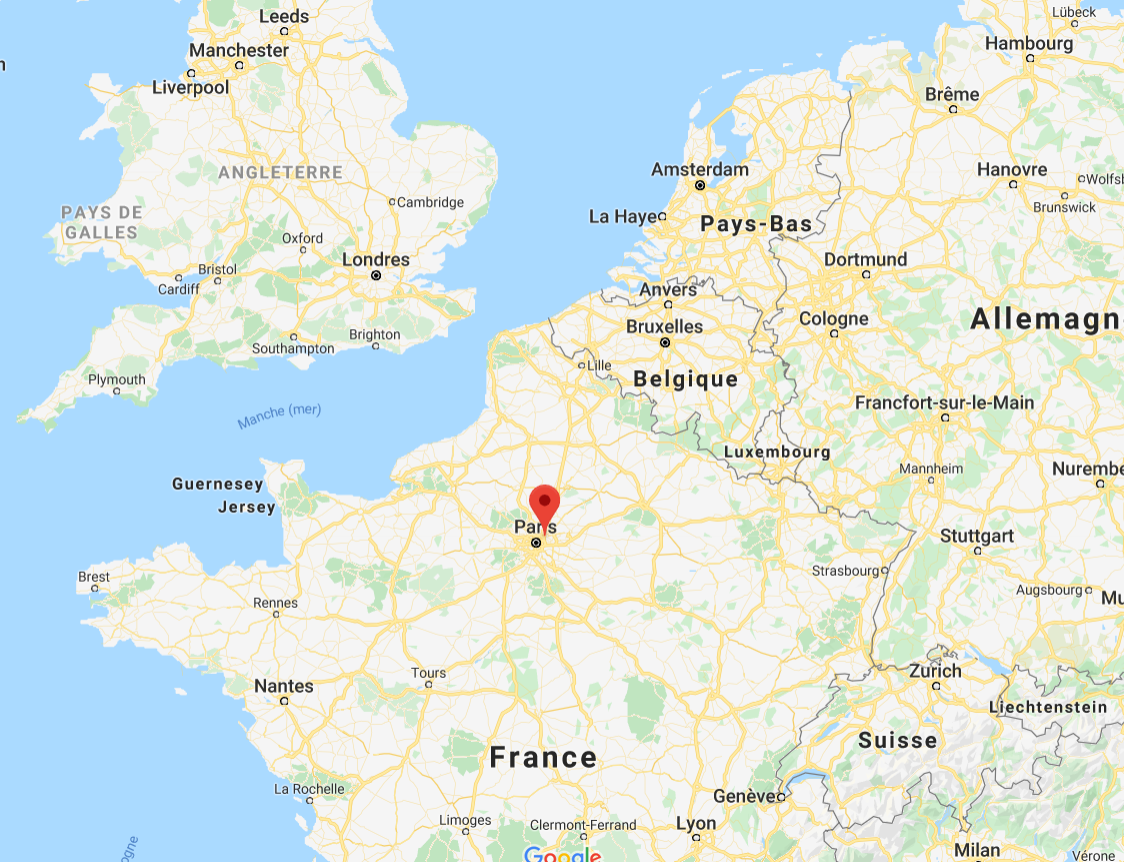
\includegraphics[width=\linewidth]{bondy}
\end{center}
\chapter{Obtaining subpoints}
In order to obtain the subpoints of the satellite, we could either use the emphem module or the following formulas : \\
\underline{Latitude $\varphi$} :
$$
\varphi = \arcsin[\sin(i)\cdot \sin(\nu + \omega)]
$$
\underline{Longitude $\lambda$} :
$$
\lambda = \arctan[\tan(\omega + \nu)\cdot \cos(i)] - \bigg[\frac{\Omega_E}n (E-e\cdot\sin(E) - \frac{\Omega_E}{n}\cdot (E_N - e\cdot\sin(E_n))\bigg]
$$
As for the elevation and the azimuth relative to the observer, we can use the following equations  :
\underline{Elevation $E$} :
$$
 E = \arccos(\frac rR \sin(\phi))\\
 \cos(\phi) = \cos L \cdot \cos \varphi \cos l + \sin \varphi \sin l
$$
\underline{Azimuth $a$} :
$$
\sin(a) = \frac{\sin L \cos \varphi}{\sin \phi}
$$
For simplicity reasons, we will use the built-in functions for both the subplot and the computing of the elevation and azimuth with respect to the observer.
\chapter{Tracking the satellite}
\begin{center}
	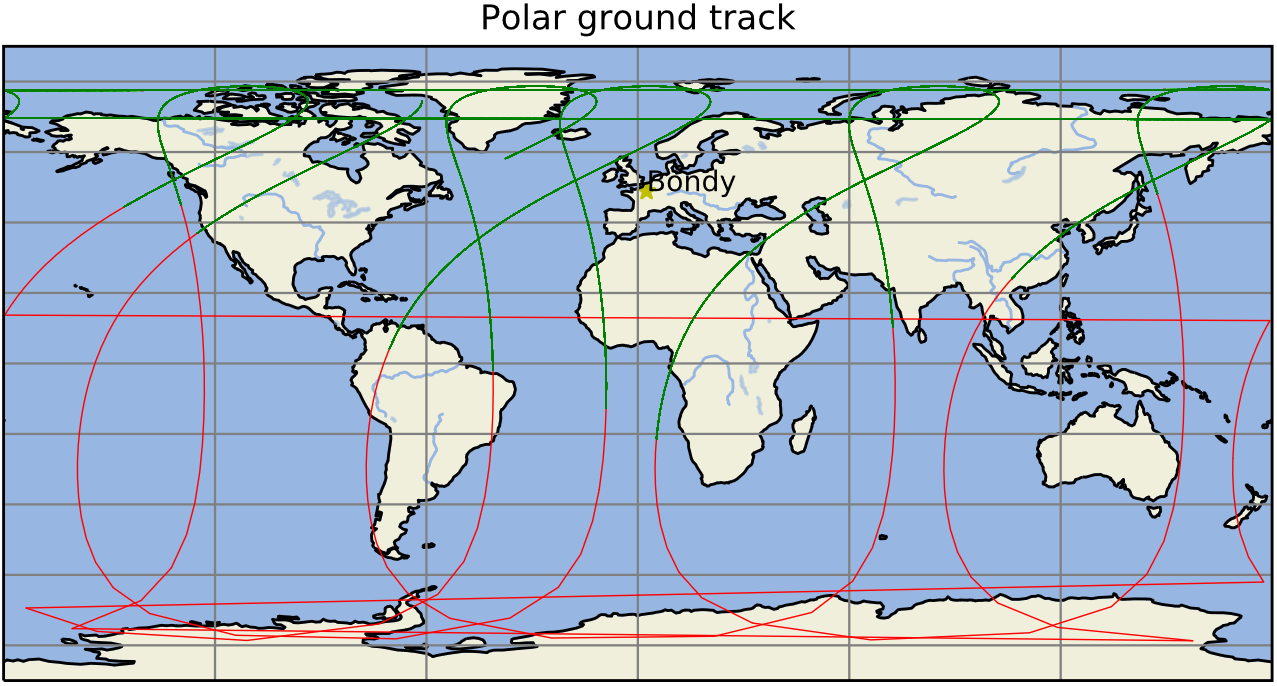
\includegraphics[width=\linewidth]{groundtrack}\\
	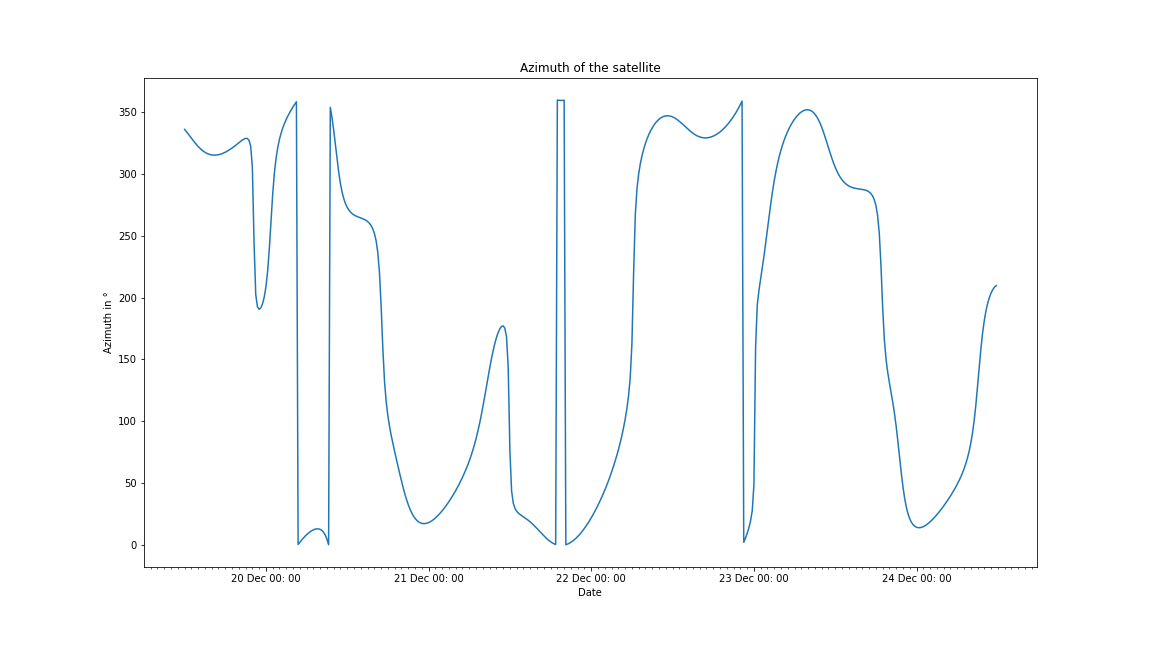
\includegraphics[width=\linewidth]{azimuth}\\
	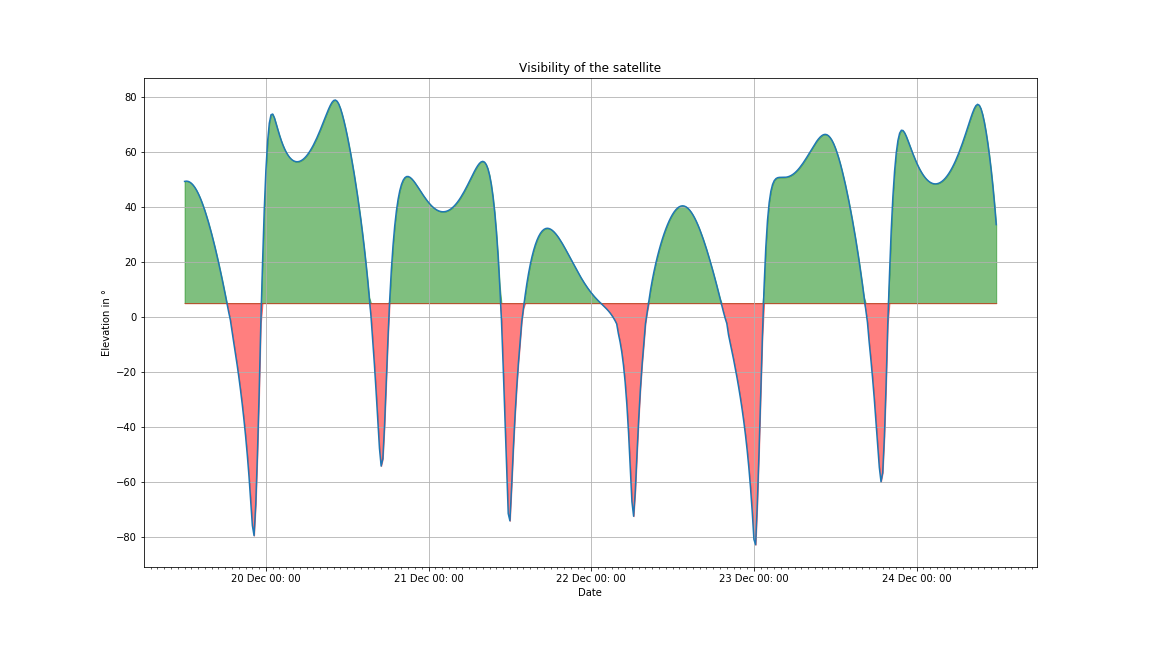
\includegraphics[width=\linewidth]{elevation}
\end{center}
\appendix




%\glsaddall
%\printglossaries

%\nocite{*}

	
%	\bibliographystyle{plain} % Le style est mis entre accolades.
%	\bibliography{references} % mon fichier de base de données s'appelle bibli.bib

%\printbibliography



%\include{lexique_an_fr}
%\listoffigures

%\listoftables
%\nopagebreak
%\include{annexes}

%\printindex

\end{document}
